\documentclass[letterpaper, 10pt, DIV=13]{scrartcl}
\usepackage[T1]{fontenc}
\usepackage[english]{babel}
\usepackage{amsmath, amsfonts, amsthm, xfrac}
\usepackage{listings}
\usepackage{color}
\usepackage{longtable}
\usepackage{qtree}

\numberwithin{equation}{section}
\numberwithin{figure}{section}
\numberwithin{table}{section}

\usepackage{sectsty}
\allsectionsfont{\normalfont\scshape} % Make all section titles in default font and small caps.

\usepackage{fancyhdr} % Custom headers and footers
\pagestyle{fancyplain} % Makes all pages in the document conform to the custom headers and footers

\fancyhead{} % No page header - if you want one, create it in the same way as the footers below
\fancyfoot[L]{} % Empty left footer
\fancyfoot[C]{} % Empty center footer
\fancyfoot[R]{\thepage} % Page numbering for right footer

\renewcommand{\headrulewidth}{0pt} % Remove header underlines
\renewcommand{\footrulewidth}{0pt} % Remove footer underlines
\setlength{\headheight}{13.6pt} % Customize the height of the header

\setlength\parindent{0pt}
\pagenumbering{gobble}

\title {
	\normalfont
	\huge{Lab 5} \\
	\vspace{10pt}
	\large{CMPT 432 - Spring 2023 | Dr. Labouseur}
}

\author{\normalfont Josh Seligman | joshua.seligman1@marist.edu}

\pagenumbering{arabic}

\definecolor{mygreen}{rgb}{0,0.6,0}
\definecolor{mygray}{rgb}{0.5,0.5,0.5}
\definecolor{mymauve}{rgb}{0.58,0,0.82}
\lstset{
  backgroundcolor=\color{white},   % choose the background color
  basicstyle=\footnotesize,        % size of fonts used for the code
  breaklines=true,                 % automatic line breaking only at whitespace
  captionpos=b,                    % sets the caption-position to bottom
  commentstyle=\color{mygreen},    % comment style
  escapeinside={\%*}{*},          % if you want to add LaTeX within your code
  keywordstyle=\color{blue},       % keyword style
  stringstyle=\color{mymauve},     % string literal style
}

\begin{document}
\maketitle

\section{Alan Question}
Describe in detail what is happening in the diagram below.
\begin{figure}[ht]
    \centering
    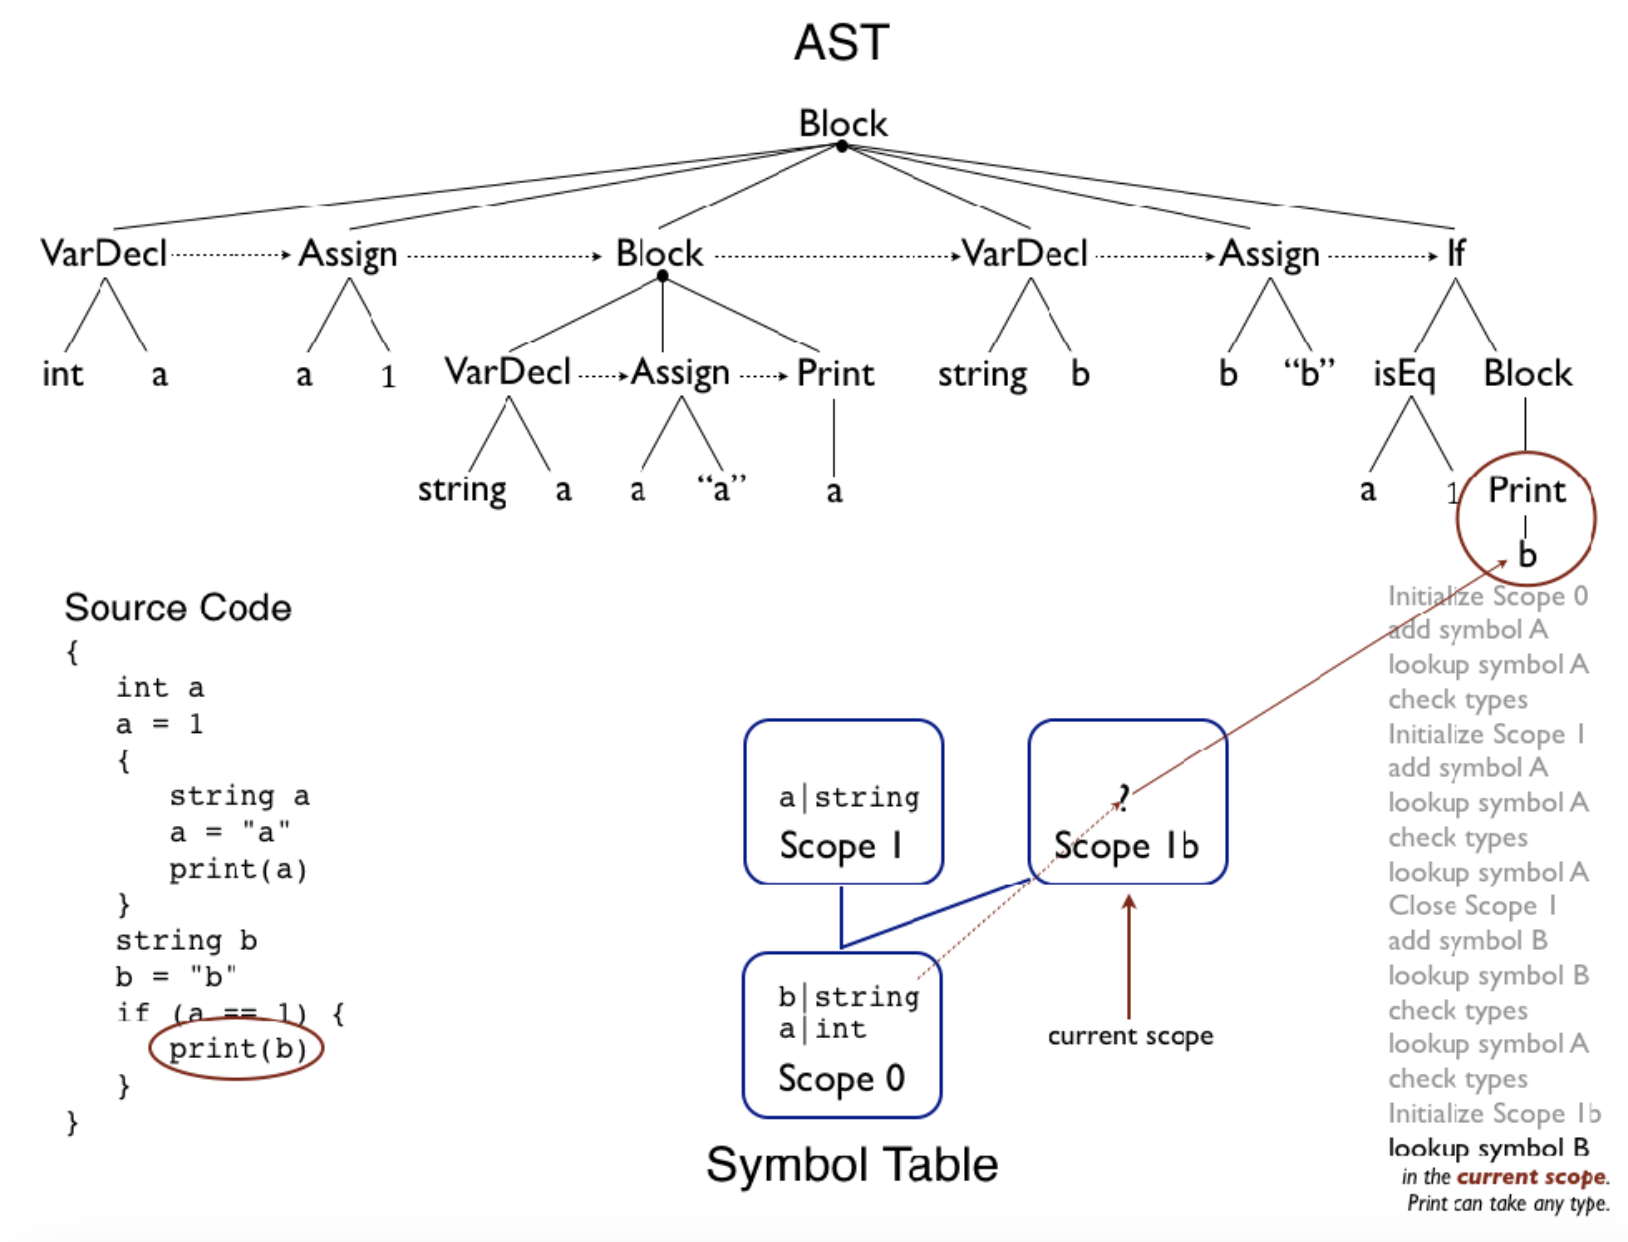
\includegraphics[height=10cm]{question}
\end{figure}
\\ \\
In the diagram, the semantic analyzer is determining if $b$ is a valid variable
within the print statement in scope 1b. To make this determination, the semantic
analyzer will look at the hashmap for scope 1b to find $b$. Unfortunately, $b$ was
not declared in the scope, so the semantic analyzer then has to check the parent
of scope 1b, which is scope 0. Fortunately, $b$ was declared in scope 0, so the
print statement is valid. However, if $b$ was not in scope 0, then an undeclared
variable error would have to be thrown.
\end{document}
